\section{Kalibrierung des Torsions-Magnetometers}

Die Messwerte der Kalibrierungsmessung sind in Abbildung \ref{fig:MPKalibrierung} zu sehen. Zur Auswertung wird zunächst der durch die Spulen fließende Strom mit dem Spulenkennwert $s$ und der Formel
\begin{equation}
 B=s\cdot I=I\cdot \eb{26,5}{nT}{mA} 
\end{equation}
in das Magnetfeld umgerechnet. Der Plot der Messwerte und der linearen Regression ist in Abbildung \ref{fig:kalibrierung} zu sehen. Bei der Regression ergab sich eine Steigung von $\eb{-0.0039}{Skt}{nT}$. Der negative Kehrwert dieser Steigung liefert den Kalibrierungsfaktor
\begin{equation}
 \frac{\tau}{|\vec{m}|}=\eb{253}{nT}{Skt} \fullstop
\end{equation}

\begin{figure}[!ht]
 \centering
 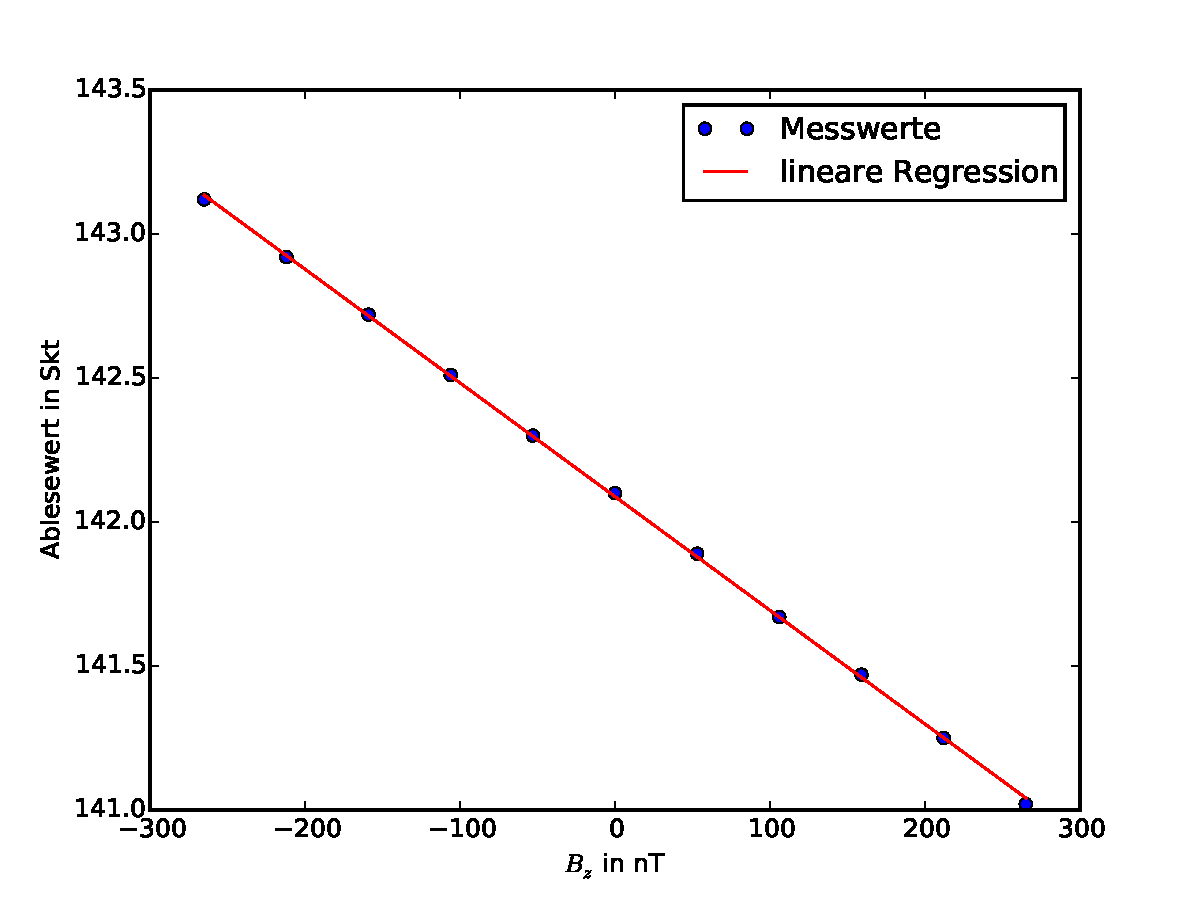
\includegraphics[width=\textwidth]{fig/kalibrierung.pdf}
 \caption[Bestimmung des Kalibrierungsfaktors des Torsions-Magnetometers]{Bestimmung des Kalibrierungsfaktors des Torsions-Magnetometers. Aufgetragen sind die Ablesewerte am Gfz in Skt über die angelegte magnetische Flussdichte in nT.}
 \label{fig:kalibrierung}
\end{figure}

\section{Kartierung}

In Abbildung \ref{fig:Kartierung} ist das Ergebnis der Kartierung abgebildet. Der Basaltgang ist deutlich als magnetische Anomalie zu sehen (in der Abbildung in rot dargestellt). Diese verläuft parallel zur Diagonalen M1-M3. Es bestätigt sich also auch nochmal die Wahl der Lage der Profile entlang von M4-M2 senkrecht zum Gang, die noch genauer untersucht wurden.

\begin{figure}[!ht]
 \centering
 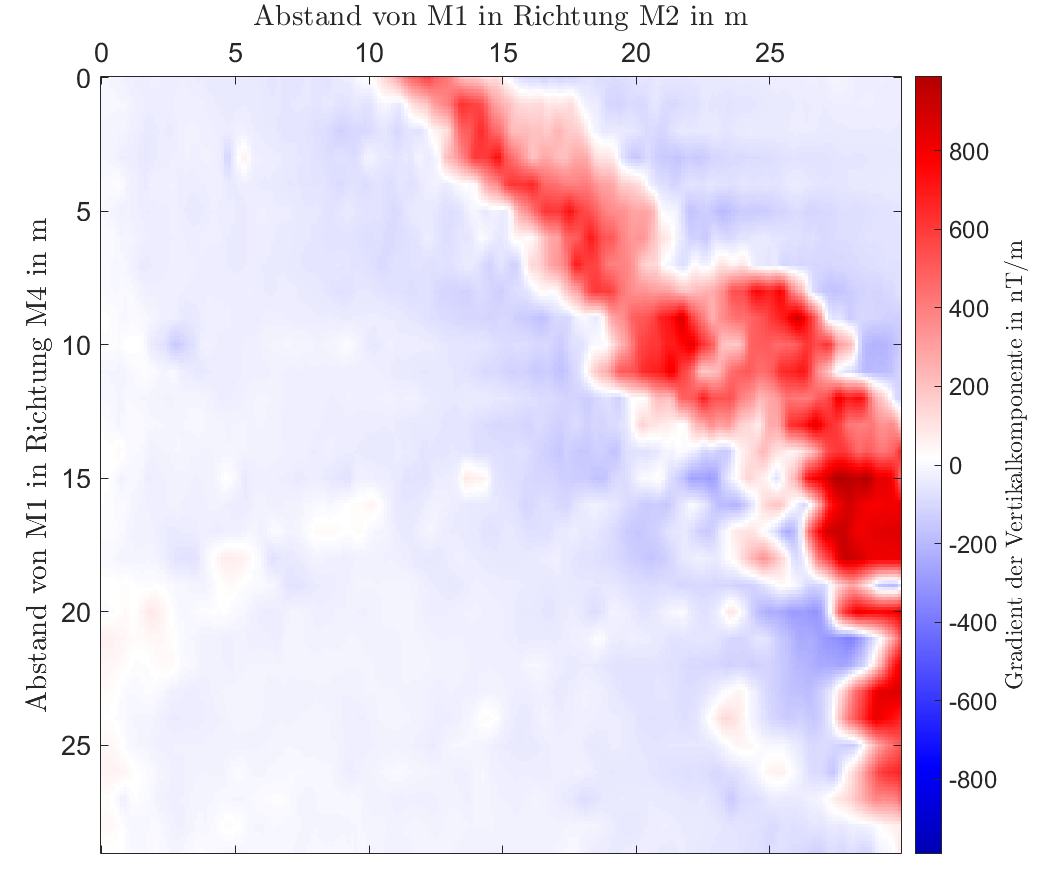
\includegraphics[width=\textwidth]{fig/kartierung_verschwommen.png}
 \caption[Ergebnis der Kartierung]{Ergebnis der Kartierung. M1 befindet sich in der linken oberen Ecke, M2 in der rechten oberen, M3 in der rechten unteren und M4 in der linken unteren.}
 \label{fig:Kartierung}
\end{figure}

\section{Vergleich der Messgeräte}

Das Messprotokoll zum Vergleich der Messgeräte befindet sich in Abbildung \ref{fig:MPVergleich} im Anhang. Die Mittelwerte dieser Messungen stehen in Tabelle \ref{tab:VergleichErgebnis}. Es fällt auf, dass das vom neuen Gerät gemessene Magnetfeld 869\,nT bzw. 897.5\,nT von den anderen Geräten abweicht. Die beiden älteren Protonenmagnetometer weichen mit 28,5\,nT deutlich weniger voneinander ab. Solche kleinen Abweichungen könnten an ungenauen Messungen der Lamorfrequenz liegen, wenn beispielsweise die Beobachtungszeit zu gering war, also nicht genug Periode vermessen wurden. Außerdem könnte die geräteinterne Zeitskala nicht ganz korrekt gewesen sein. Auch die Stangen der Messgeräte hatten vielleicht nicht genau die selbe Länge oder die Messgeräte wurden nicht genau in Richtung Nord-Süd ausgerichtet. Diese Gründe können jedoch vermutlich nicht die größeren Abweichung vom neueren Gerät zu den anderen erklären.

\begin{table}[!ht]
 \centering
 \caption{Messergebnis des Vergleichs der Protonenmagnetometer und des Fluxgates}
 \begin{tabular}{rl}
 \toprule
 Messgerät & Totalintensität an Basisstation in nT \\
 \midrule
 Nr. 1 & 48102 \\
 Nr. 2 & 48073,5 \\
 Neues Gerät & 48971 \\
 Fluxgate &  \\
 \bottomrule
 \end{tabular}
\label{tab:VergleichErgebnis}
\end{table}

Um die Messungen der verschiedenen Messgeräte miteinander vergleichen zu können, muss eines ausgewählt werden, auf das die Messungen mit den anderen korrigiert werden. Dazu verwenden wir die Messungen des Magnetfelds am BFO (siehe Abbildung \ref{fig:BFO}). Aus diesem Diagramm ist abzulesen, dass die Totalintensität des Magnetfelds am BFO am Messtag, den 22.05.2018, von 12:00 Uhr bis 18:00 Uhr zwischen 48220\,nT und 48250\,nT betrug. Die Messwerte des Geräts Nr. 1 liegen am nächsten an diesen, weswegen wir alle Werte auf dieses korrigieren. Es wird also für alle folgenden Auswertungen auf alle Messungen mit Gerät Nr. 2  28,5\,nT addiert und von allen Messungen mit dem neuen Gerät werden 869\,nT subtrahiert.

\section{Profile}

Es wurden 


% \begin{figure}
%  \centering
%  \includegraphics[width=\textwidth]{fig/}
%  \caption{}
%  \label{fig:}
% \end{figure}